% Copyright 2016 - 2017 Bas van Meerten and Wouter Franssen
%
%This file is part of ssNake.
%
%ssNake is free software: you can redistribute it and/or modify
%it under the terms of the GNU General Public License as published by
%the Free Software Foundation, either version 3 of the License, or
%(at your option) any later version.
%
%ssNake is distributed in the hope that it will be useful,
%but WITHOUT ANY WARRANTY; without even the implied warranty of
%MERCHANTABILITY or FITNESS FOR A PARTICULAR PURPOSE.  See the
%GNU General Public License for more details.
%
%You should have received a copy of the GNU General Public License
%along with ssNake. If not, see <http://www.gnu.org/licenses/>.

\documentclass[11pt,a4paper]{article}
% Copyright 2016 - 2017 Bas van Meerten and Wouter Franssen
%
%This file is part of ssNake.
%
%ssNake is free software: you can redistribute it and/or modify
%it under the terms of the GNU General Public License as published by
%the Free Software Foundation, either version 3 of the License, or
%(at your option) any later version.
%
%ssNake is distributed in the hope that it will be useful,
%but WITHOUT ANY WARRANTY; without even the implied warranty of
%MERCHANTABILITY or FITNESS FOR A PARTICULAR PURPOSE.  See the
%GNU General Public License for more details.
%
%You should have received a copy of the GNU General Public License
%along with ssNake. If not, see <http://www.gnu.org/licenses/>.

\usepackage[british]{babel}
\usepackage{graphicx,booktabs,listings,amsmath,pgfplots,pgfplotstable}
\usepackage[small,bf,nooneline]{caption}
\usepackage{subcaption}
\usepackage[sort&compress,numbers]{natbib}
\usepackage{tikz}
\usepackage{mathtools}
\usepackage[nottoc]{tocbibind}%adds bibliography to table of contents.
\graphicspath{{./images/}}
%\setlength{\textwidth}{453pt} %597 pt is the a4 paperwidth. Minus 2 in margin. 72 pt = 1 in
%\setlength{\hoffset}{-\oddsidemargin}
%\setlength{\voffset}{-30pt} %
%\setlength{\textheight}{651 pt} %a4 height 845 pt minus 2* total headheight. In this case 2*88pt
%% examine margines via the layout package. Use command \layout{} in document to draw a picture.
%\setlength{\parindent}{0.5 cm}
%\setlength{\parskip}{0 cm}
\usepackage[left=82pt,right=82pt,top=95pt,bottom=95pt,footnotesep=0.5cm]{geometry}
%\setlength{\headheight}{14pt}

%define colours--------------------
%dark
\usepackage{xcolor}
\definecolor{MyGrayD}{RGB}{1,1,1}
\definecolor{MyRedD}{RGB}{237,45,46}
\definecolor{MyGreenD}{RGB}{0,140,71}
\definecolor{MyBlueD}{RGB}{24,89,169}
\definecolor{MyOrangeD}{RGB}{243,125,34}
\definecolor{MyPurpleD}{RGB}{102,44,145}
\definecolor{MyBrownD}{RGB}{161,29,32}
\definecolor{MyPinkD}{RGB}{179,56,147}
%normal
\definecolor{MyGray}{RGB}{114,114,114}
\definecolor{MyRed}{RGB}{241,89,95}
\definecolor{MyGreen}{RGB}{121,195,106}
\definecolor{MyBlue}{RGB}{89,154,211}
\definecolor{MyOrange}{RGB}{249,166,90}
\definecolor{MyPurple}{RGB}{158,102,171}
\definecolor{MyBrown}{RGB}{205,112,88}
\definecolor{MyPink}{RGB}{215,127,179}
%light
\definecolor{MyGrayL}{RGB}{204,204,204}
\definecolor{MyRedL}{RGB}{242,174,172}
\definecolor{MyGreenL}{RGB}{216,228,170}
\definecolor{MyBlueL}{RGB}{184,210,235}
\definecolor{MyOrangeL}{RGB}{242,209,176}
\definecolor{MyPurpleL}{RGB}{212,178,211}
\definecolor{MyBrownL}{RGB}{221,184,169}
\definecolor{MyPinkL}{RGB}{235,191,217}
%----------------------------------

%Figure ref with hyperref
\newcommand{\fref}[1]{\hyperref[#1]{Figure \ref*{#1}}}
\newcommand{\sref}[1]{\hyperref[#1]{Section \ref*{#1}}}
\newcommand{\tref}[1]{\hyperref[#1]{Table \ref*{#1}}}

%Makes a new command for figures with input values: filename, width(times linewidth),
% caption and label.
\newcommand{\onefigure}[4]{
\setlength{\captionwidth}{#2\linewidth}
\begin{figure}
\includegraphics[width=#2\linewidth]{#1}
\centering
\parbox{\linewidth}{\caption{#3}
\label{#4}}
\end{figure}
}

%Makes a new command for tikz figures with input values: tikz commands, 
% caption and label.
\newcommand{\onetikz}[3]{
\settowidth{\captionwidth}{#1}
\ifthenelse{\lengthtest{\captionwidth<0.7\linewidth}}{\setlength{\captionwidth}{0.7\linewidth}}{}

\begin{figure}
\centering
#1
\centering
\parbox{\linewidth}{\caption{#2}
\label{#3}}
\end{figure}
}

%Makes a new command for two figures next to each other with input values: filename1, caption1, label1,filename2, caption2 and label2. Figure width is set to 0.47\linewidth and the space between the figures is filled with \hfill so the sides of the figures align with to edge of the line.
\newcommand{\twofigure}[6]{
\setlength{\captionwidth}{\linewidth}
\begin{figure*}[ht!]
\begin{minipage}[t]{0.47\linewidth}
\includegraphics[width=\linewidth]{#1}
\centering
\caption{#2}
\label{#3}
\end{minipage}
\hfill
\begin{minipage}[t]{0.47\linewidth}
\centering
\includegraphics[width= \linewidth]{#4}
\centering
\caption{#5}
\label{#6}
\end{minipage}
\end{figure*}
}


%Makes a new command for a table with caption witdh equal to the total table width. Input: tabular, caption and label. Example:
%\onetable{
%\begin{tabular}{ccc}
%a&b&c\\
%\hline
%1&1&1\\
%1&1&1\\
%1&1&1\\
%\end{tabular}
%{The caption.}
%{tab:table1}
%}
\newcommand{\onetable}[3]{
\settowidth{\captionwidth}{#1}
\ifthenelse{\lengthtest{\captionwidth<0.7\linewidth}}{\setlength{\captionwidth}{0.7\linewidth}}{}
\begin{table}
\caption{#2}
\vspace{-0.24cm} %Puts caption close to toprule
\label{#3}
\centering
#1
\end{table}
}

%Makes a long table with captionwidth equal to tablewidth. It takes the following arguments:
%1: Column specifier (e.g. cccc)
%2: Caption
%3: Label
%4: First head (i.e. first row of regular table)
%5: Head of consecutive pages
%6: Foot of pagebreak
%7: Lastfoot (e.g. \midrule)
%8: Body of table
\newcommand{\onelongtable}[8]{
\begin{center}
\settowidth{\captionwidth}{
\begin{tabular}{#1}
#4
#8
\end{tabular}} % This ends the captionwidth part. Next comes the real table.

\begin{longtable}{#1}
\caption{#2}\\
\vspace{-0.74cm} %Puts caption close to toprule
\label{#3}\\

#4
\endfirsthead

#5
\endhead

#6
\endfoot

#7
\endlastfoot

#8
\end{longtable}
\end{center}}




%1:pgfplots code
%2:width
%3:caption
%4:label
\newcommand{\pgfplotsfigure}[4]{
\pgfplotsset{width=#2\linewidth}
\setlength{\captionwidth}{#2\linewidth}
\begin{figure}[t]
\centering
#1
\centering
\parbox{\linewidth}{\caption{#3}
\label{#4}}
\end{figure}
}


\usepackage[bitstream-charter]{mathdesign}
\usepackage[T1]{fontenc}
\usepackage[protrusion=true,expansion,tracking=true]{microtype}
\pgfplotsset{compat=1.7,/pgf/number format/1000 sep={}, axis lines*=left,axis line style={gray},every outer x axis line/.append style={-stealth'},every outer y axis line/.append style={-stealth'},tick label style={font=\small},label style={font=\small},legend style={font=\footnotesize}}
\usepackage{colortbl}
\usetikzlibrary{calc}

%Set section font
\usepackage{sectsty}
\allsectionsfont{\color{black!70}\fontfamily{SourceSansPro-LF}\selectfont}
%--------------------


%Set toc fonts
\usepackage{tocloft}
%\renewcommand\cftchapfont{\fontfamily{SourceSansPro-LF}\bfseries}
\renewcommand\cfttoctitlefont{\color{black!70}\Huge\fontfamily{SourceSansPro-LF}\bfseries}
\renewcommand\cftsecfont{\fontfamily{SourceSansPro-LF}\selectfont}
%\renewcommand\cftchappagefont{\fontfamily{SourceSansPro-LF}\bfseries}
\renewcommand\cftsecpagefont{\fontfamily{SourceSansPro-LF}\selectfont}
\renewcommand\cftsubsecfont{\fontfamily{SourceSansPro-LF}\selectfont}
\renewcommand\cftsubsecpagefont{\fontfamily{SourceSansPro-LF}\selectfont}
%--------------------

%Define header/foot
%\usepackage{fancyhdr}
%\pagestyle{fancy}
%\fancyhead[LE,RO]{\fontfamily{SourceSansPro-LF}\selectfont \thepage}
%\fancyhead[LO,RE]{\fontfamily{SourceSansPro-LF}\selectfont \leftmark}
%\fancyfoot[C]{}
%--------------------

%remove page number from first chapter page
%\makeatletter
%\let\ps@plain\ps@empty
%\makeatother
%----------------------

\usepackage[hidelinks,colorlinks,allcolors=black, pdftitle={DQSQ},pdfauthor={Wouter M.J.\ Franssen}]{hyperref}

\interfootnotelinepenalty=10000 %prevents splitting of footnote over multiple pages
\linespread{1.2}

\title{\color{black}\fontfamily{SourceSansPro-LF}\bfseries 2D double-quantum/single-quantum (SQ/DQ)
correlation spectroscopy analysis in ssNake}
\author{}
\date{\color{black}\fontfamily{SourceSansPro-LF}\bfseries \today}


\begin{document}
%\newgeometry{left=72pt,right=72pt,top=95pt,bottom=95pt,footnotesep=0.5cm}
\microtypesetup{protrusion=true} % enables protrusion

\maketitle

\section{Introduction}
This tutorial will demonstrate how 2D double-quantum single-quantum NMR data can be processed in ssNake.
The tutorial delivered with the ssNake program is considered as prior knowledge.
If you have not yet studied this, please do so before continuing with this example.

In liquid state NMR, homonuclear correlations (e.g.\ $^{1}$H-$^1$H) are commonly recorded using a COSY experiment.
This experiment uses the scalar couplings (J-couplings) between nuclei to transfer magnetization, and to obtain information on the connectivity between the spins.
Another way to do this, is to use dipolar couplings, and perform a NOESY experiment.
In solid state samples, scalar couplings are often too weak for COSY experiments (as the relaxation times are much shorter), and other types of experiments should be performed.
A common 2D homonuclear solid state experiment is a double-quantum single-quantum experiment.
In this experiment, the direct dimension contains information on single-quantum transitions, while the indirect dimension contains the double quantum transition information. 

When two spins A and B are connected (via a dipolar coupling), they give rise to crosspeaks in the DQSQ experiment.
In the DQ dimension, A and B will have a resonances at double the Larmor frequency (because of the double quantum character).
If there is a sizable dipolar coupling between A and B, there will also be crosspeaks at the sum frequency ($\delta_\text{A} + \delta_\text{B}$).
The intensity of these peaks compared to the main (diagonal) peaks provides information on the strength of the dipolar coupling.

\section{Data}
The data we will use in this tutorial is of a $^1$H--$^1$H DQSQ experiment performed on methylammonium lead iodide (CH$_3$NH$_3$PbI$_3$), a perovskite material used in a new generation of solar cells.
The spectrum was recorded on a Varian 400 MHz machine, using a 3.2 mm rotor and 15 kHz MAS.


\section{Processing}
Processing a DQSQ experiment is quite similar to regular 2D data processing.
The main difference lies in the referencing of the double quantum  dimension.

\begin{itemize}
  \item Open the data delivered with this tutorial in ssNake via Open $\longrightarrow$ File
	\item Zero fill the data to 4096 points (Matrix $\longrightarrow$ Sizing, and fill in 4096 at the
	  size and leave the offset as is)
	\item Push the `Fourier' button to transform the data to a spectrum
	\item Phase the spectrum using only zero order phasing
\end{itemize}
This should result in something like this:
\begin{center}
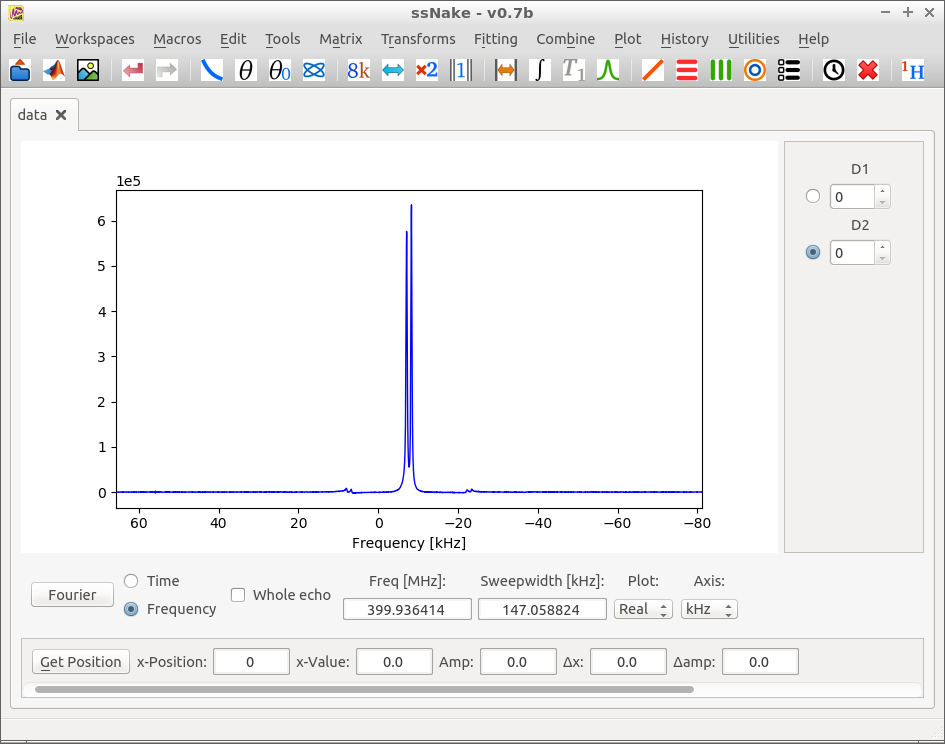
\includegraphics[width=0.7\linewidth]{Figs/Fig1.png}
\end{center}
And zoomed on the main peaks:
\begin{center}
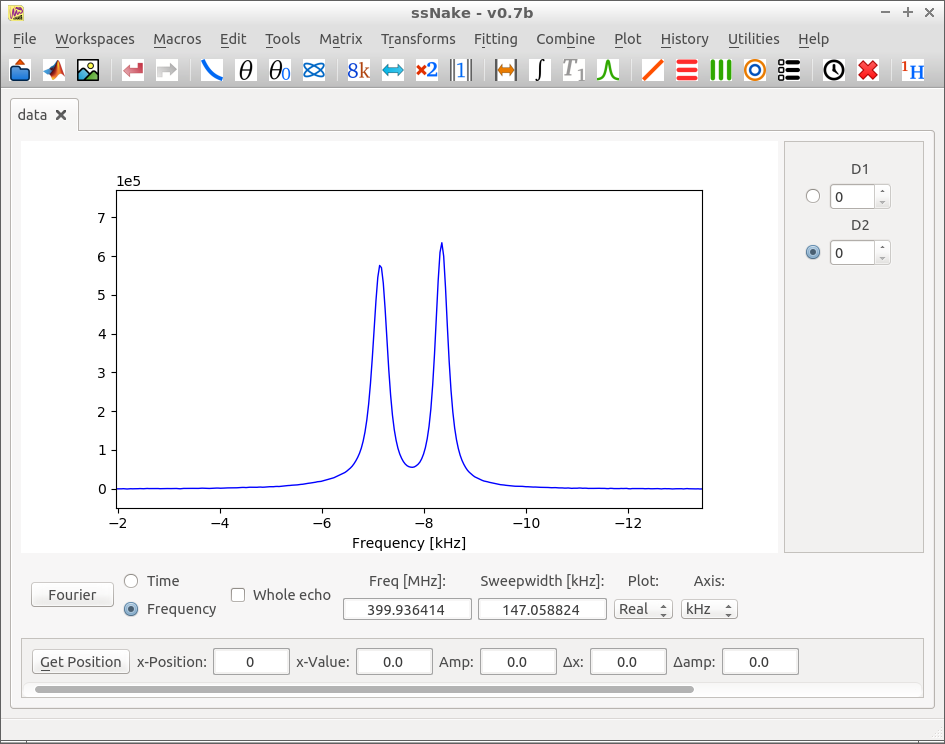
\includegraphics[width=0.7\linewidth]{Figs/Fig2.png}
\end{center}
This shows the first trace of our 2D data.
We have now processed the direct dimension (D2), we now continue with the indirect dimension (D1).

\begin{itemize}
  \item Get the position of the rightmost main peak (so that we can view it along D1). Use `Get
	 Position', and click on the peak. This give x-Position = 2030 (or a value close to that).
  \item Put this value in the D2 box of the side frame and press `Enter'
\end{itemize}
This now shows the time evolution along the indirect dimension:
\begin{center}
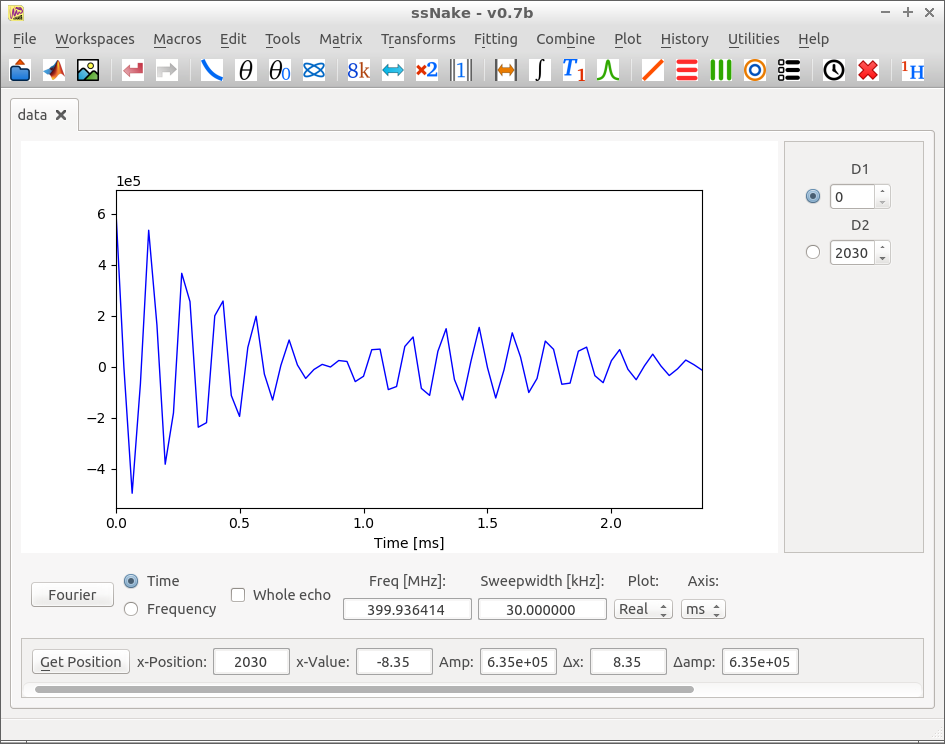
\includegraphics[width=0.7\linewidth]{Figs/Fig3.png}
\end{center}
This data was recorded using a hypercomplex scheme (states--TPPI), and requires a conversion:

\begin{itemize}
  \item Use Transforms $\longrightarrow$ Hypercomplex $\longrightarrow$ States--TPPI to convert it
	\item Use Tools $\longrightarrow$ Complex conjugate to invert the sense of direction to the
	  ssNake definition \footnote{Most Varian sequences define the sense of the rotation in the
	  indirect dimension in the opposite way as we do it. This is, however, dependent on the way the
	used pulse-sequence is written, so we cannot correct this for you automatically. Without this
 step, the spectrum along D1 will appear flipped. }
\end{itemize}
This should result in:
\begin{center}
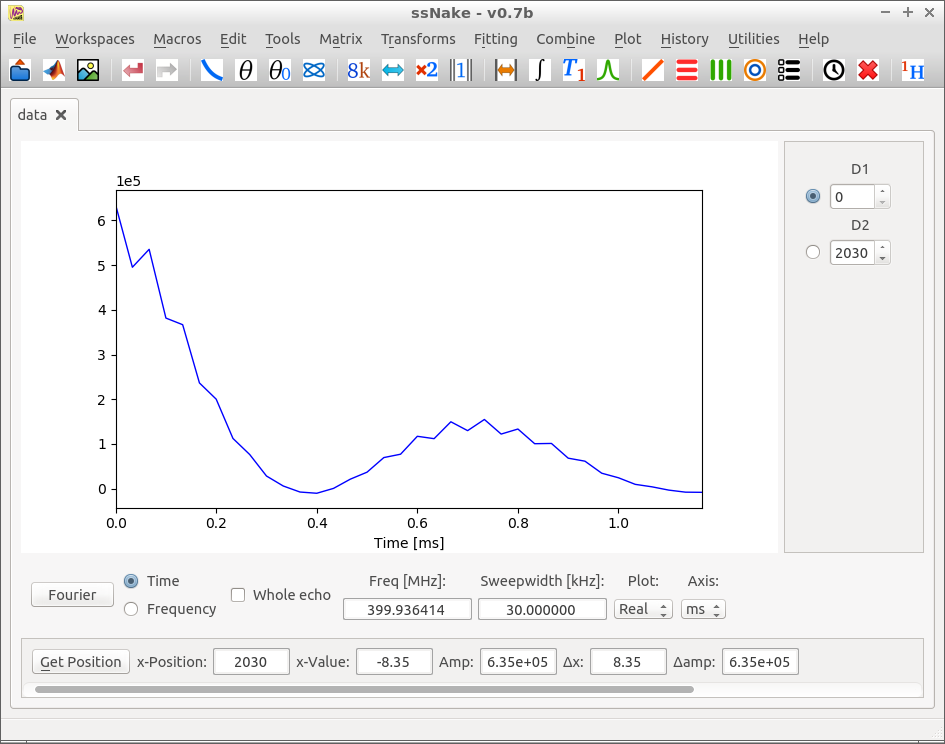
\includegraphics[width=0.7\linewidth]{Figs/Fig4.png}
\end{center}

\begin{itemize}
  \item Zero fill to 512 points
  \item Fourier transform
  \item Phase using 0 order only
\end{itemize}
The spectrum along the indirect dimension should now look like:
\begin{center}
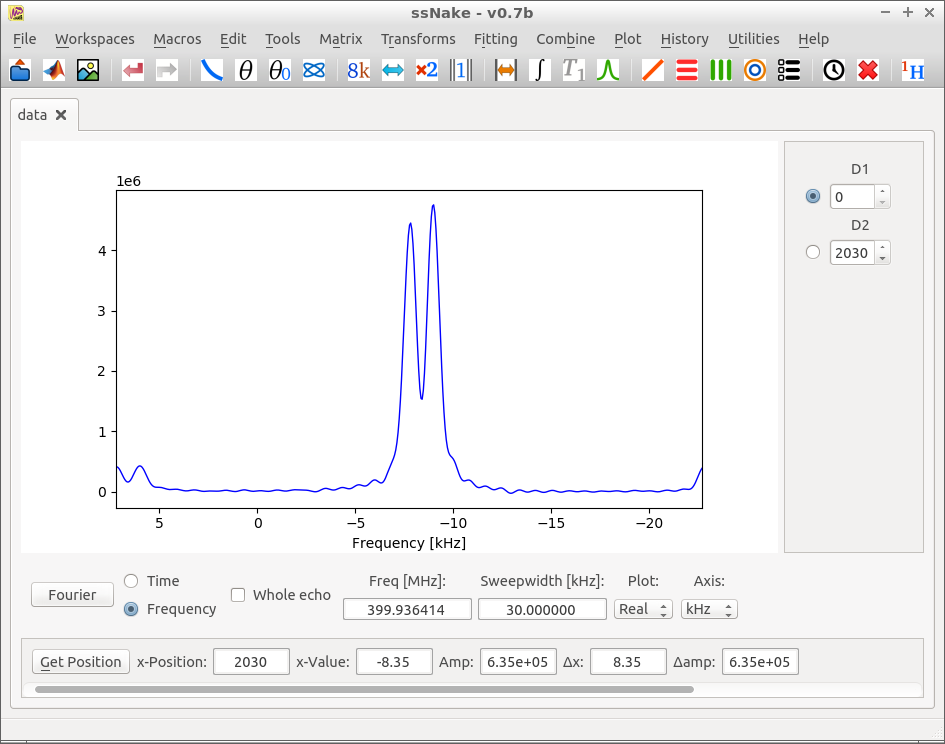
\includegraphics[width=0.7\linewidth]{Figs/Fig5.png}
\end{center}

We now need to set the correct chemical shift reference for both dimensions.
The reference frequency (0 ppm) is  399.9344480 MHz (based on an external reference).
We can just apply this value to the direct dimension (D2):


\begin{itemize}
  \item Go to D2 (use the radio button in the side frame)
  \item Use Tools $\longrightarrow$ Reference $\longrightarrow$ Set Reference, and fill in
	 399.9344480 for the frequency (and leave the other values unchanged).
  \item Set the current view to `ppm' (in the bottom frame with `Axis')
\end{itemize}
This results in:

\begin{center}
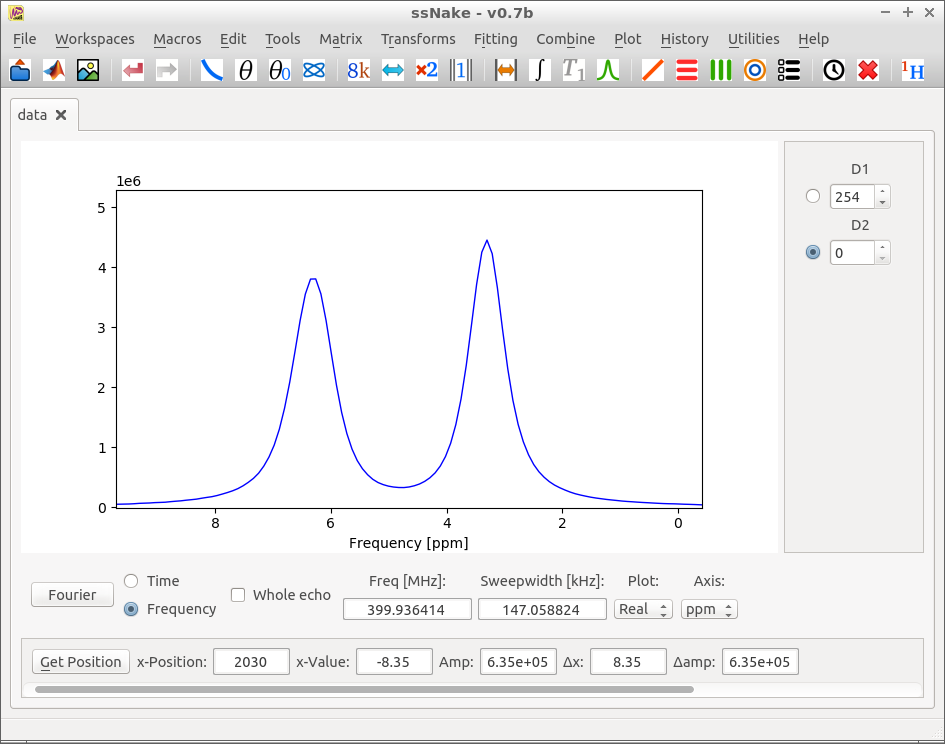
\includegraphics[width=0.7\linewidth]{Figs/Fig6.png}
\end{center}

Now we continue with D1.
The tricky part with referencing a double-quantum dimension is that our external reference is not correct anymore: all frequencies are doubled in this dimension.
This means that our zero ppm frequency (399.9344480 MHz) is different in D1: its difference with
respect to the carrier frequency should be doubled.
In our case, the carrier frequency (centre of the spectrum) is 399.936414 MHz (see the bottom frame).
The difference with this and the reference frequency is -0.0019659 MHz. This value should be added to the reference frequency (this makes the new reference frequency to be twice as far away from the carrier frequency as before).
The reference frequency in D1 is thus equal to  $399.9344480 -0.0019659 = 399.9324820$ MHz.

\begin{itemize}
  \item Go to D1 (use the radio button in the side frame)
  \item Use Tools $\longrightarrow$ Reference $\longrightarrow$ Set Reference, and fill in
399.9324820 MHz
  \item Set the axis to `ppm' (in the bottom frame with `Axis')
  \item Go back to D2 (radio button)
\end{itemize}
Now, we are finished processing, and it is time to view our 2D spectrum.
Use Plot $\longrightarrow$ Contour to create a contour plot.
Zoomed in, this looks like (with the lower contour level at 55 \%, see the side frame, contour levels can be zoomed with `shift + scroll') :

\begin{center}
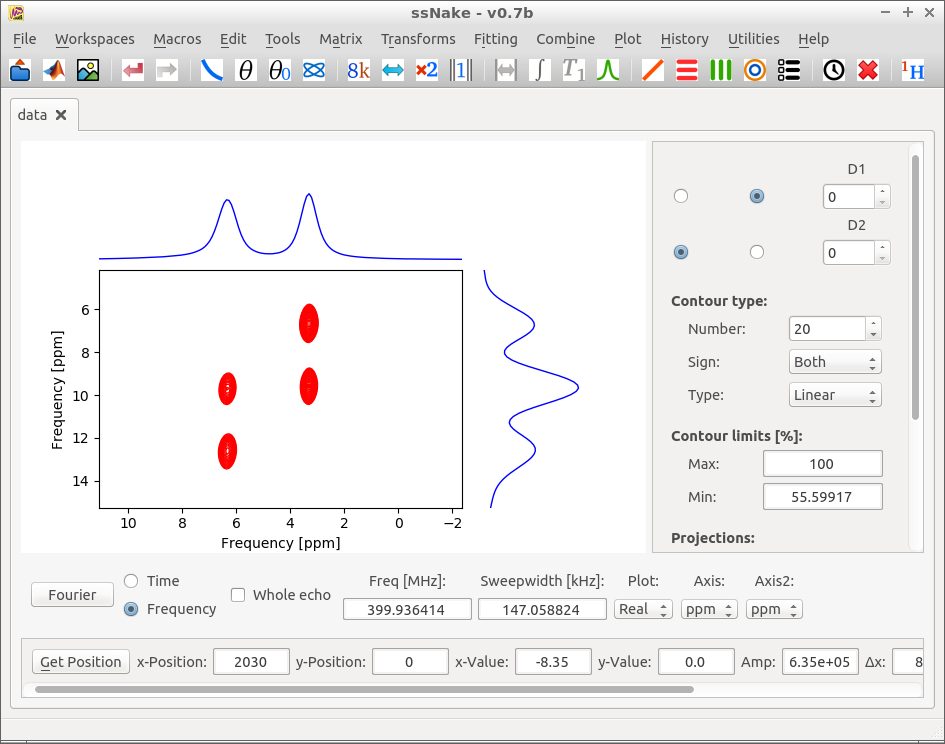
\includegraphics[width=0.7\linewidth]{Figs/Fig7.png}
\end{center}
From this spectrum it is clear that the two peaks are connected.
Both have an cross peak in D1 at $\approx 10$ ppm, as well as self peaks at twice there single quantum chemical shift.
These self peaks are located on the diagonal, which ssNake can also draw.
In the side frame tick `Diagonal' and set the multiplier to 2 (we want the diagonal to have a slope of 2, because of the double-quantum character).
This results in:

\begin{center}
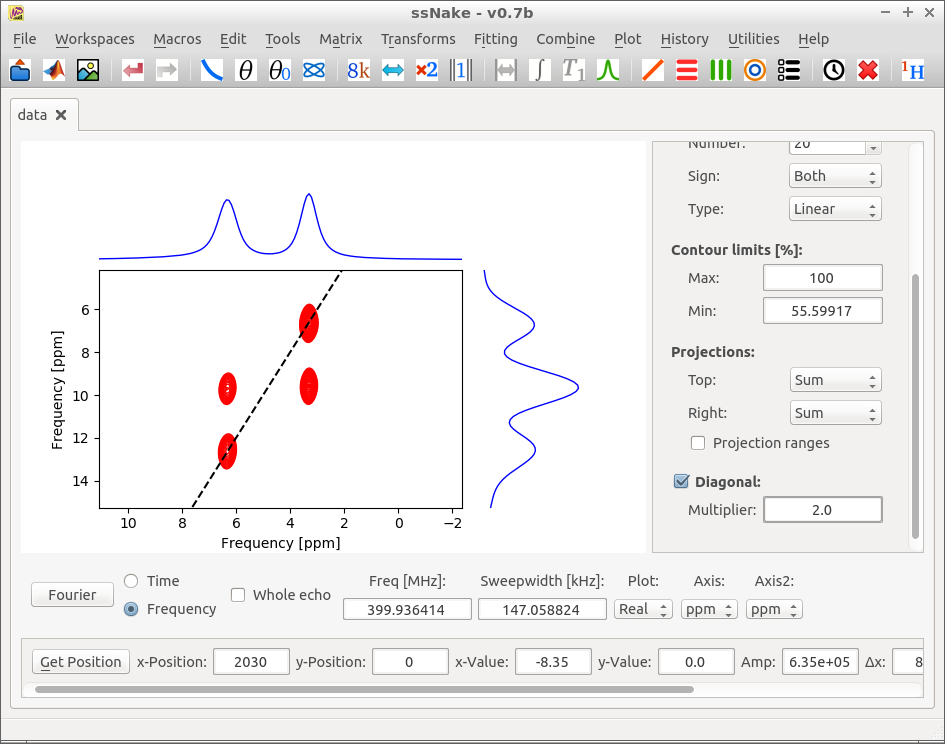
\includegraphics[width=0.7\linewidth]{Figs/Fig8.png}
\end{center}
Which is the final spectrum.
The pattern that is shown here is common for a DQSQ experiment, when two chemical species are connected via a dipolar coupling.
This spectrum is also delivered together with this tutorial (as a .mat file).
Note that in the D2 dimension the width has been reduced to the relevant part via Matrix $\longrightarrow$ Extract Part.
This was done to reduced the size of the saved data.



\end{document}
